\documentclass[11pt]{article}
\usepackage[a4paper,margin=22mm,headheight=16pt]{geometry}
\usepackage{fontspec,xeCJK,xcolor,graphicx,enumitem,fancyhdr,titlesec}
\usepackage{hyperref}
\IfFontExistsTF{Times New Roman}{\setmainfont{Times New Roman}}{\setmainfont{TeX Gyre Termes}}
\IfFontExistsTF{FangSong}{\setCJKmainfont[AutoFakeBold=2]{FangSong}}{\IfFontExistsTF{仿宋}{\setCJKmainfont[AutoFakeBold=2]{仿宋}}{\IfFontExistsTF{FandolFang-Regular.otf}{\setCJKmainfont[AutoFakeBold=2]{FandolFang-Regular.otf}}{\setCJKmainfont{FandolSong-Regular.otf}}}}
\definecolor{ink}{HTML}{173747}\definecolor{accent}{HTML}{227E82}
\hypersetup{colorlinks=true,urlcolor=accent,linkcolor=accent}
\linespread{1.22}\setlength{\parindent}{0pt}\setlength{\parskip}{6pt}
\setlist[itemize]{leftmargin=1.4em,itemsep=3pt}
\titleformat{\section}{\large\bfseries\color{ink}}{}{0pt}{}
\titlespacing*{\section}{0pt}{14pt}{7pt}
\pagestyle{fancy}\fancyhf{}\lhead{\small LEARNPATH / 学习手册}\rhead{\small Source-grounded learning}\cfoot{\small\thepage}
\emergencystretch=2em\widowpenalty=10000\clubpenalty=10000
\newcommand{\Needspace}[1]{\par\begingroup\dimen0=#1\relax\vskip0pt plus\dimen0\penalty-100\vskip0pt plus-\dimen0\vskip\dimen0\penalty9999\vskip-\dimen0\vskip0pt\endgroup}
\begin{document}


{\LARGE\bfseries\color{ink} 工具权限与用户确认}\par

2026-10-08 | Day03/30 | 阅读 8 分钟 + 练习 3 分钟\par\vspace{6pt}

\Needspace{5\baselineskip}\section*{今日导航}

今天回答：用户说“帮我安排”，是否意味着可以直接支付？目标是区分能力、权限和本次授权，并设计一个具体的确认点。先回忆昨日混合方案：哪些步骤可以探索，哪些动作必须受到确定约束？

\Needspace{5\baselineskip}\section*{会调用不等于被允许调用}

工具告诉系统怎样读取或改变外部状态；权限限定它可以访问的范围；本次授权说明用户具体要求做什么。拥有付款工具，不代表用户每次咨询都授权付款。一个工具描述再清楚，也不能替代产品侧的访问控制。

MCP 的指定版本规范讨论工具与资源的连接及安全原则；协议能帮助标准化连接，却不会自动保证业务动作正确。[S4] 这里引用的是明确版本的原则，不把它称为当前所有平台的统一实现。

\begin{center}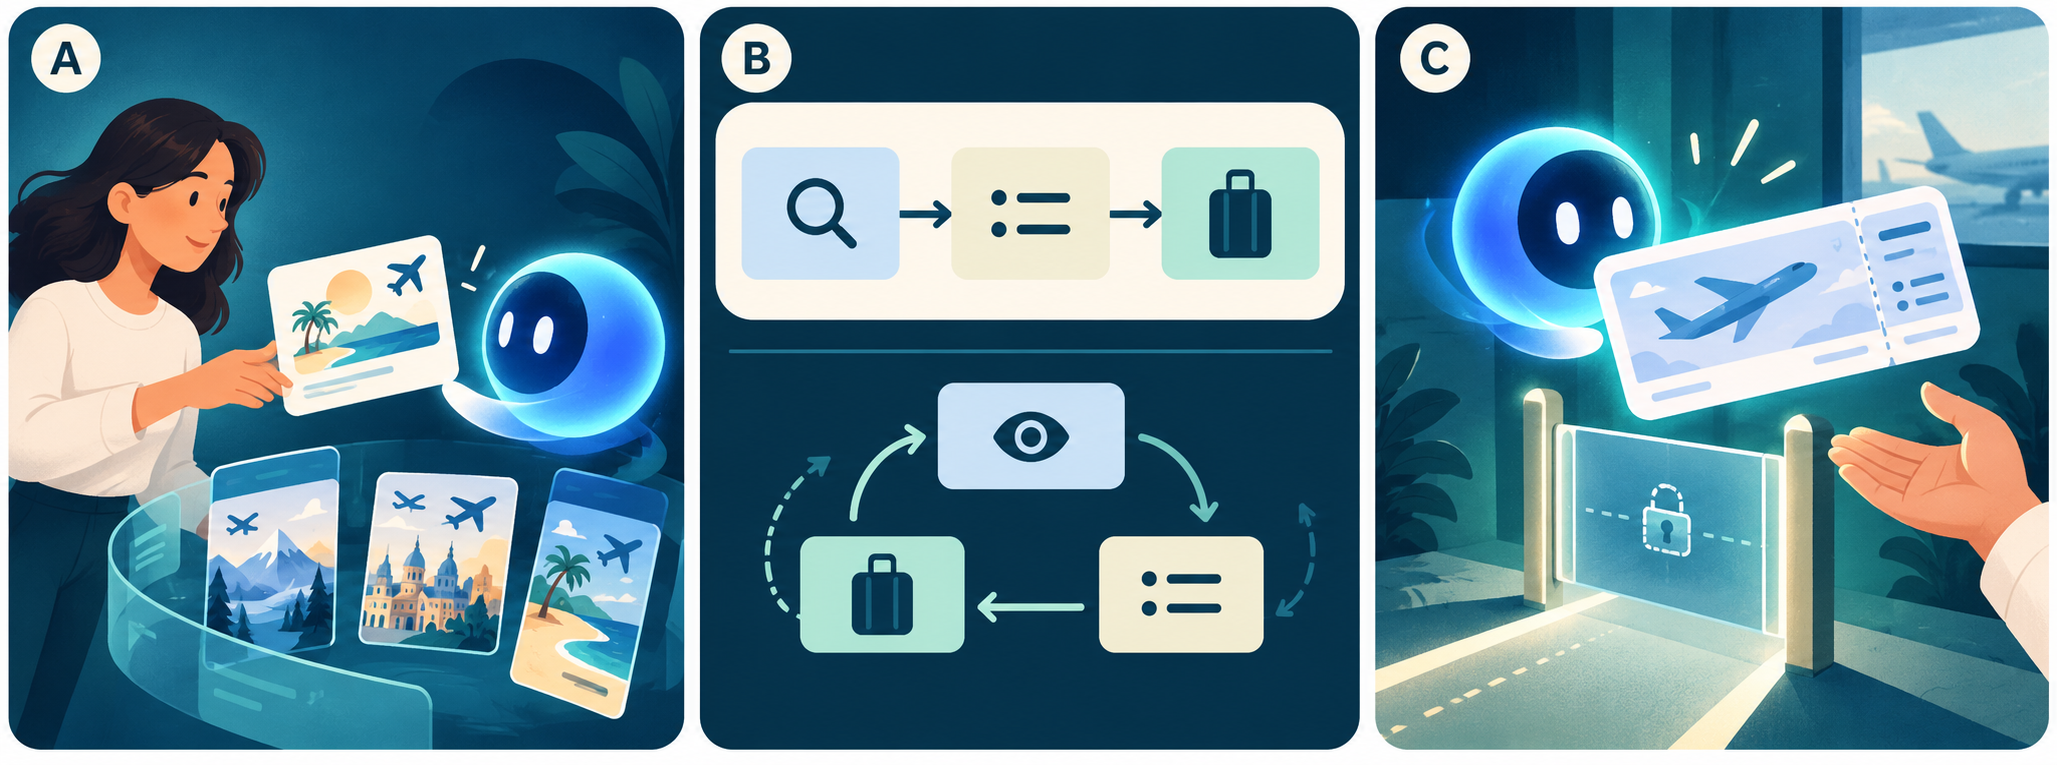
\includegraphics[width=\linewidth,height=0.26\textheight,keepaspectratio]{../assets/figure-8284fa500410.png}\par

{\small 本课重点看 C 区。A 明确委托目标；B 比较固定步骤与观察反馈循环；C 在提交购买前设置人的确认。示意图不代表真实产品界面。}\par

{\footnotesize AI生成教学示意，非实物照片、原始史料或官方架构。生成方式：内置文生图；提示词见仓库 docs/image-prompts.json。}\end{center}

\Needspace{5\baselineskip}\section*{把读、准备与提交分开}

查询候选通常读取信息；生成订单草稿准备改变状态；支付或发送会对外产生结果。这些动作的后果不同，适合不同的确认强度。工具设计资料强调明确的用途和返回信息，本课把它落实为用户可理解的动作边界。[S2]

图 C 的门位于候选与最终购买之间。确认应让用户看见具体对象、金额、时间、重要条件和即将发生的动作，而不是只问“是否继续”。如果确认后价格变化或对象更换，原确认不再完整覆盖新动作，应重新取得针对变化内容的同意。

可撤销不等于没有成本。取消订单可能产生费用，邮件撤回可能失败。设计权限时，应依据真实后果与用户意图，而不是仅依据界面是否有一个撤销按钮。

\Needspace{5\baselineskip}\section*{教学案例：避免重复购买}

假设提交订单后网络超时，界面没有收到成功消息。此时不能直接推断购买失败并再提交一次。先查询订单状态，再决定恢复动作；若无法确认，向用户说明不确定性。这里讨论的是一般设计原则，不是具体支付接口实现。

用户看到的状态应区分“草稿已准备”“等待确认”“提交中”“结果未知”和“已确认完成”。这能让失败恢复有依据。最终验收既检查票是否符合要求，也检查是否在授权范围内、是否发生重复提交。评估框架要包含异常轨迹，而不能只测一路顺利的样例。[S3]

\Needspace{5\baselineskip}\section*{三分钟练习与面试自查}

写一条具体的购买前确认文案，包含对象、总金额、日期与关键条件。再写网络超时后的第一步。

参考文案：“将购买10月12日某航班的指定席位，总额为已展示的金额；请核对旅客、时间和退改规则后确认付款。”真实产品必须填入实际核验值，不能保留“某航班”等占位。超时后先查订单状态。追问：用户先前确认过另一个价格怎么办？应说明变化，不能把旧确认挪用到新价格。

\Needspace{5\baselineskip}\section*{复盘与明日连接}

可靠的 Agent 产品把能做、允许做和这次要做区分开。确认不是打断用户的固定仪式，而是让有后果的具体动作可审阅。明天把今天的状态区分展开，学习长任务如何保存进度并在失败后恢复。

\Needspace{6\baselineskip}\section*{扩展学习 / Further reading}\small 以下为选读，不计入每日必做时间。\begin{enumerate}[leftmargin=1.6em]

\item [S1] \href{https://www.anthropic.com/engineering/building-effective-agents}{Building effective agents} — 读工作流与 Agent 的区分；用作架构框架，不把旧工具清单当最新。\par Anthropic | 发布：2024-12-19 | 核验：2026-10-08

\item [S2] \href{https://www.anthropic.com/engineering/writing-tools-for-agents}{Writing effective tools for agents} — 关注工具边界、返回结果和评价方法如何影响可用性。\par Anthropic | 发布：2025-09-11 | 核验：2026-10-08

\item [S3] \href{https://www.anthropic.com/engineering/demystifying-evals-for-ai-agents}{Demystifying evals for AI agents} — 理解结果评价与执行轨迹；为后续验收指标课程准备。\par Anthropic | 发布：2026-01-09 | 核验：2026-10-08

\item [S4] \href{https://modelcontextprotocol.io/specification/2025-06-18}{Model Context Protocol specification} — 阅读指定版本的用途和安全原则；不称其为最新版本。\par MCP project | 发布：2025-06-18（指定版本） | 核验：2026-10-08

\item [S5] \href{https://adk.dev/agents/}{Agents in ADK} — 比较 LLM Agent、工作流 Agent 与自定义 Agent 的分类。\par Google ADK | 发布：未标注 | 核验：2026-10-08

\end{enumerate}

\end{document}